\documentclass[12pt]{article}
\usepackage[T2A]{fontenc}
\usepackage[utf8]{inputenc}
\usepackage{multirow}
\usepackage{caption}
\usepackage{subcaption}
\usepackage{amsmath}
\usepackage{changepage}
\usepackage{graphicx}
\usepackage{float}
\usepackage[english,russian]{babel}
\usepackage{amsmath, amsfonts, amssymb, amsthm, mathtools}
\usepackage{xcolor}
\usepackage{array}
\usepackage{hyperref}
\usepackage[top = 1.5cm, left = 1.5 cm, right = 1.5 cm, bottom = 3 cm]{geometry}
\graphicspath{ {./images/} }
 
\title{Определение $C_p/C_v методом адиабатического расширения$}
\author{Шахматов Андрей, Б02-304}
\date{\today}
  
\begin{document}
\begin{titlepage}
    \begin{center}
        {\large МОСКОВСКИЙ ФИЗИКО-ТЕХНИЧЕСКИЙ ИНСТИТУТ (НАЦИОНАЛЬНЫЙ ИССЛЕДОВАТЕЛЬСКИЙ УНИВЕРСИТЕТ)}
    \end{center}
    \begin{center}
        {\large Физтех-школа физики и исследований им. Ландау}
    \end{center}
    
    
    \vspace{3cm}
    {\huge
        \begin{center}
            \textbf{Определение Cp/Cv методом адиабатического расширения}
        \end{center}
    }
    \vspace{2cm}
    \begin{flushright}
        {\LARGE Автор:\\ Шахматов Андрей Юрьевич \\
            \vspace{0.2cm}
            Б02-304}
    \end{flushright}
    \vspace{7 cm}
    \begin{center}
        Долгопрудный 2024
    \end{center}
\end{titlepage}

% \maketitle

\begin{abstract}
    Исследовано изменение давления в сосуде с газом после адиабатического расширения. На основе полученных 
    данных определено отношение $\frac{C_p}{C_v}$ для углекислого газа.       
\end{abstract}
\tableofcontents

\section{Введение}
Цель настоящей работы заключалась в определении отношения $\frac{C_p}{C_v}$ для углекислого газа. 

\section{Методика}
Для определения отношение теплоёмкостей $\frac{C_p}{C_v}$ рассмотрим следующий процесс над газом. Сначала 
адиабатическое расширение газа от давления $p_1$ до атмосферного $p_0$, а затем изохорное 
охлаждение газа до комнатной температуры. Для описания адиабатического расширения применим следующее уравнение: 
\begin{equation}
    \left( \frac{P_1}{P_2} \right)^{\gamma - 1} = \left( \frac{T_1}{T_2} \right)^\gamma  
    \label{eq:1}
\end{equation}
После для описания изохорного охлаждения применим закон Гей-Люссака и найдём выражение для показателя адиабаты: 
\begin{equation}
    \gamma = \frac{\ln \left( \frac{P_1}{P_0} \right) }{\ln \left( \frac{P_1}{P_3} \right) }
    \label{eq:2}
\end{equation}
Теперь перейдём к описанию используемой установки (Рис. \ref{fig:u}). Используемая для опытов экспериментальня установка состоит из стеклянного сосуда А (объёмом около 20 л), снабженного краном К, и U-образного жидкостного манометра, измеряющего избыточное давление газа в сосуде. Схема установки показана на Рис. 1. 

Избыточное давление создаётся с помощью резиновой груши, сосединённой с сосудом трубкой с краном $К_1$.

В начале опыта  в стеклянном сосуде А находится исследуемый газ при комнатной температуре $T_1$ и давлении $P_1$, несколько превышающем атмосферное давление  $P_0$. После открытия крана К, соединяющего сосуд А с атмосферой, давление и температура газа будут понижаться. Это уменьшение температуры приближённо можно считать адиабатическим.
\begin{figure}[H]
    \centering
    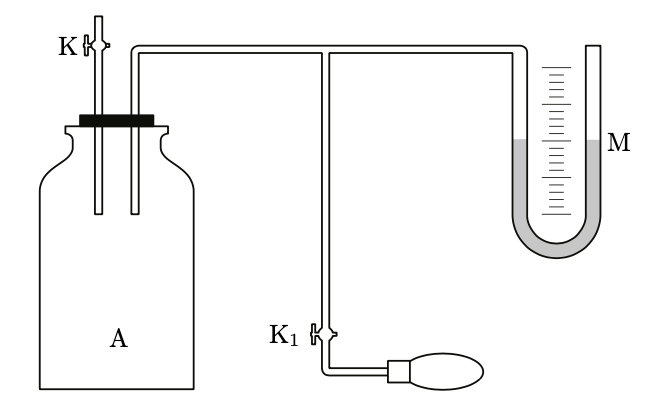
\includegraphics[width=0.7\linewidth]{1.jpg}
    \caption{Установка для определения $C_p / C_v$ методом адиабатического расширения газа}
    \label{fig:u}
\end{figure}
Тогда с учётом специфики установки возможно упростить выражение \ref{eq:2} с учётом $P = P_0 + \rho g h$ и $\rho g h \ll P_0$:  
\begin{equation}
    \gamma = \frac{C_p}{C_v} \approx \frac{h_1}{h_1 - h_2}
    \label{eq:gamma}
\end{equation}

\section{Результаты и их обсуждение}
Для того, что бы определенить время установления температур газа, было проведено измерение изменения 
уровня давления газа от времени (Таблица \ref{tab:1}). По полученным данным построен график \ref{fig:1}. 
Согласно графику можно определить время релаксации системы равным примерно $40$ с. Потому при дальнейших 
измерениях значения давлений в системе будут измеряться спустя $40$ с после проведения эксперимента.    
\begin{figure}[H]
    \centering
    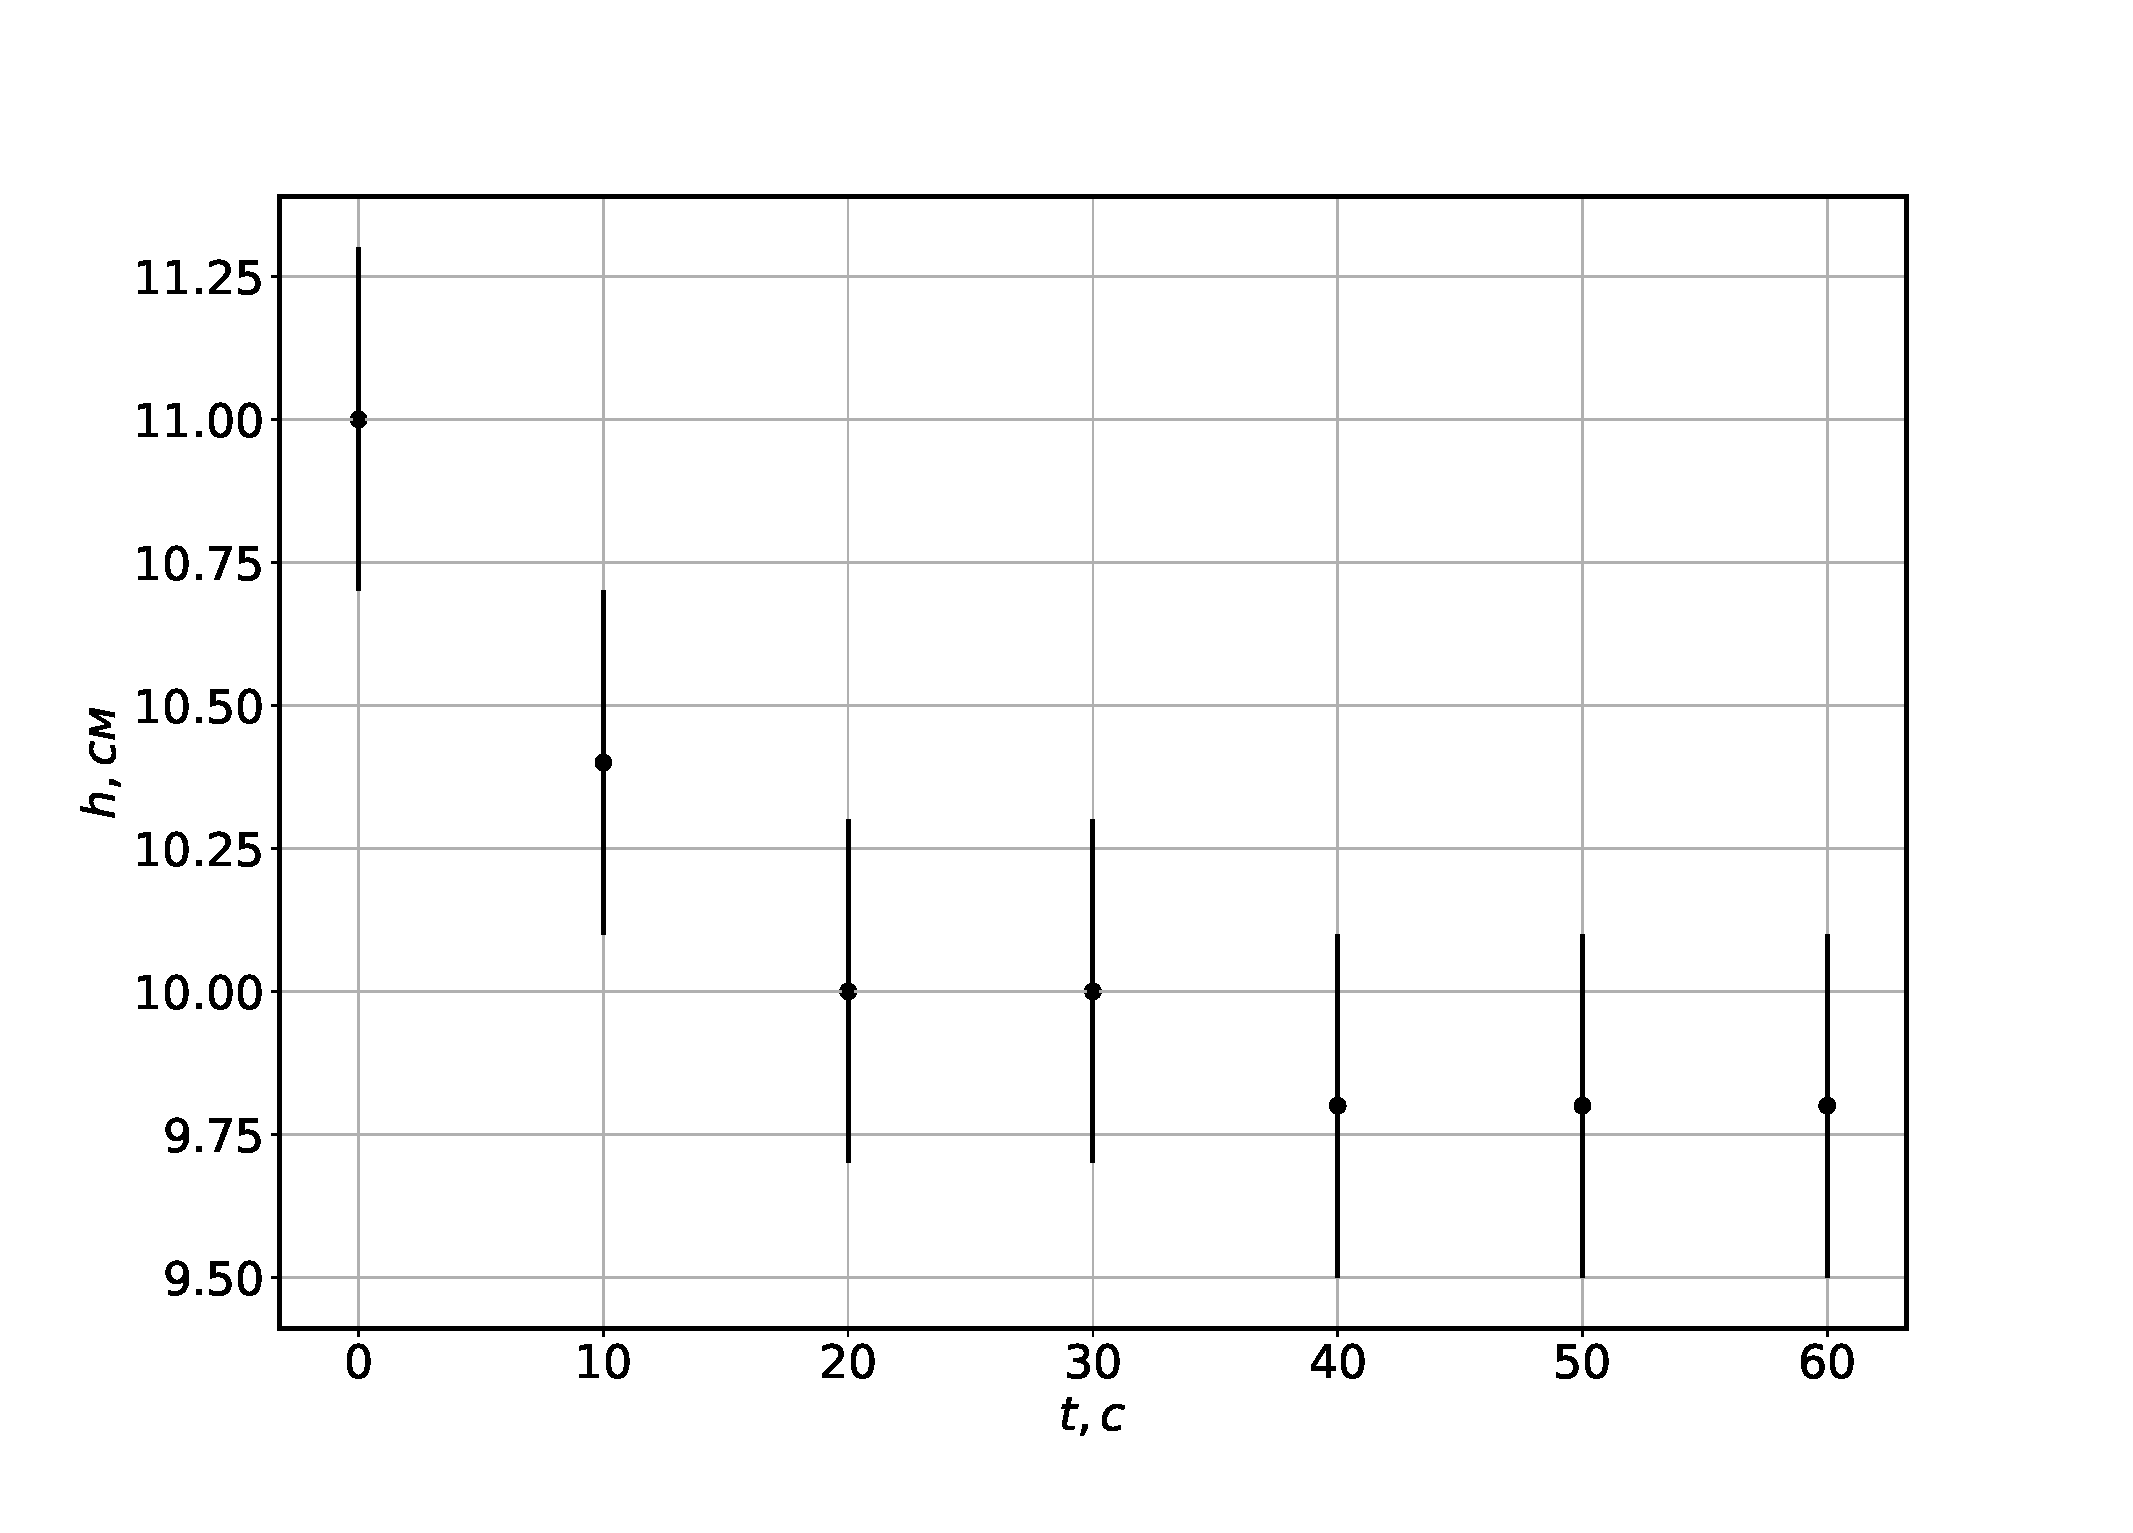
\includegraphics[width=0.7\linewidth]{ht.eps}
    \caption{Зависимость давления в сосуде $h$ от времени с момента проведения эксперимента $t$}
    \label{fig:1}
\end{figure}
Измерена зависимость давления в сосуде (высоты жидкости монометра) $h_2$ после проведения 
эксперимента описанного ранее от начального давления в сосуде $h_1$ (Таблицы \ref{tab:2} и \ref{tab:3}). 
Измерения проводились при временах открывания вентиля сосуда $1.5$ с и $5$ с. После согласно выражению 
\ref{eq:gamma} для каждого времени открытия клапана был получен показатель адиабаты $\gamma$. Полученные 
значения нанесены на график \ref{fig:2}. 
\begin{figure}[H]
    \centering
    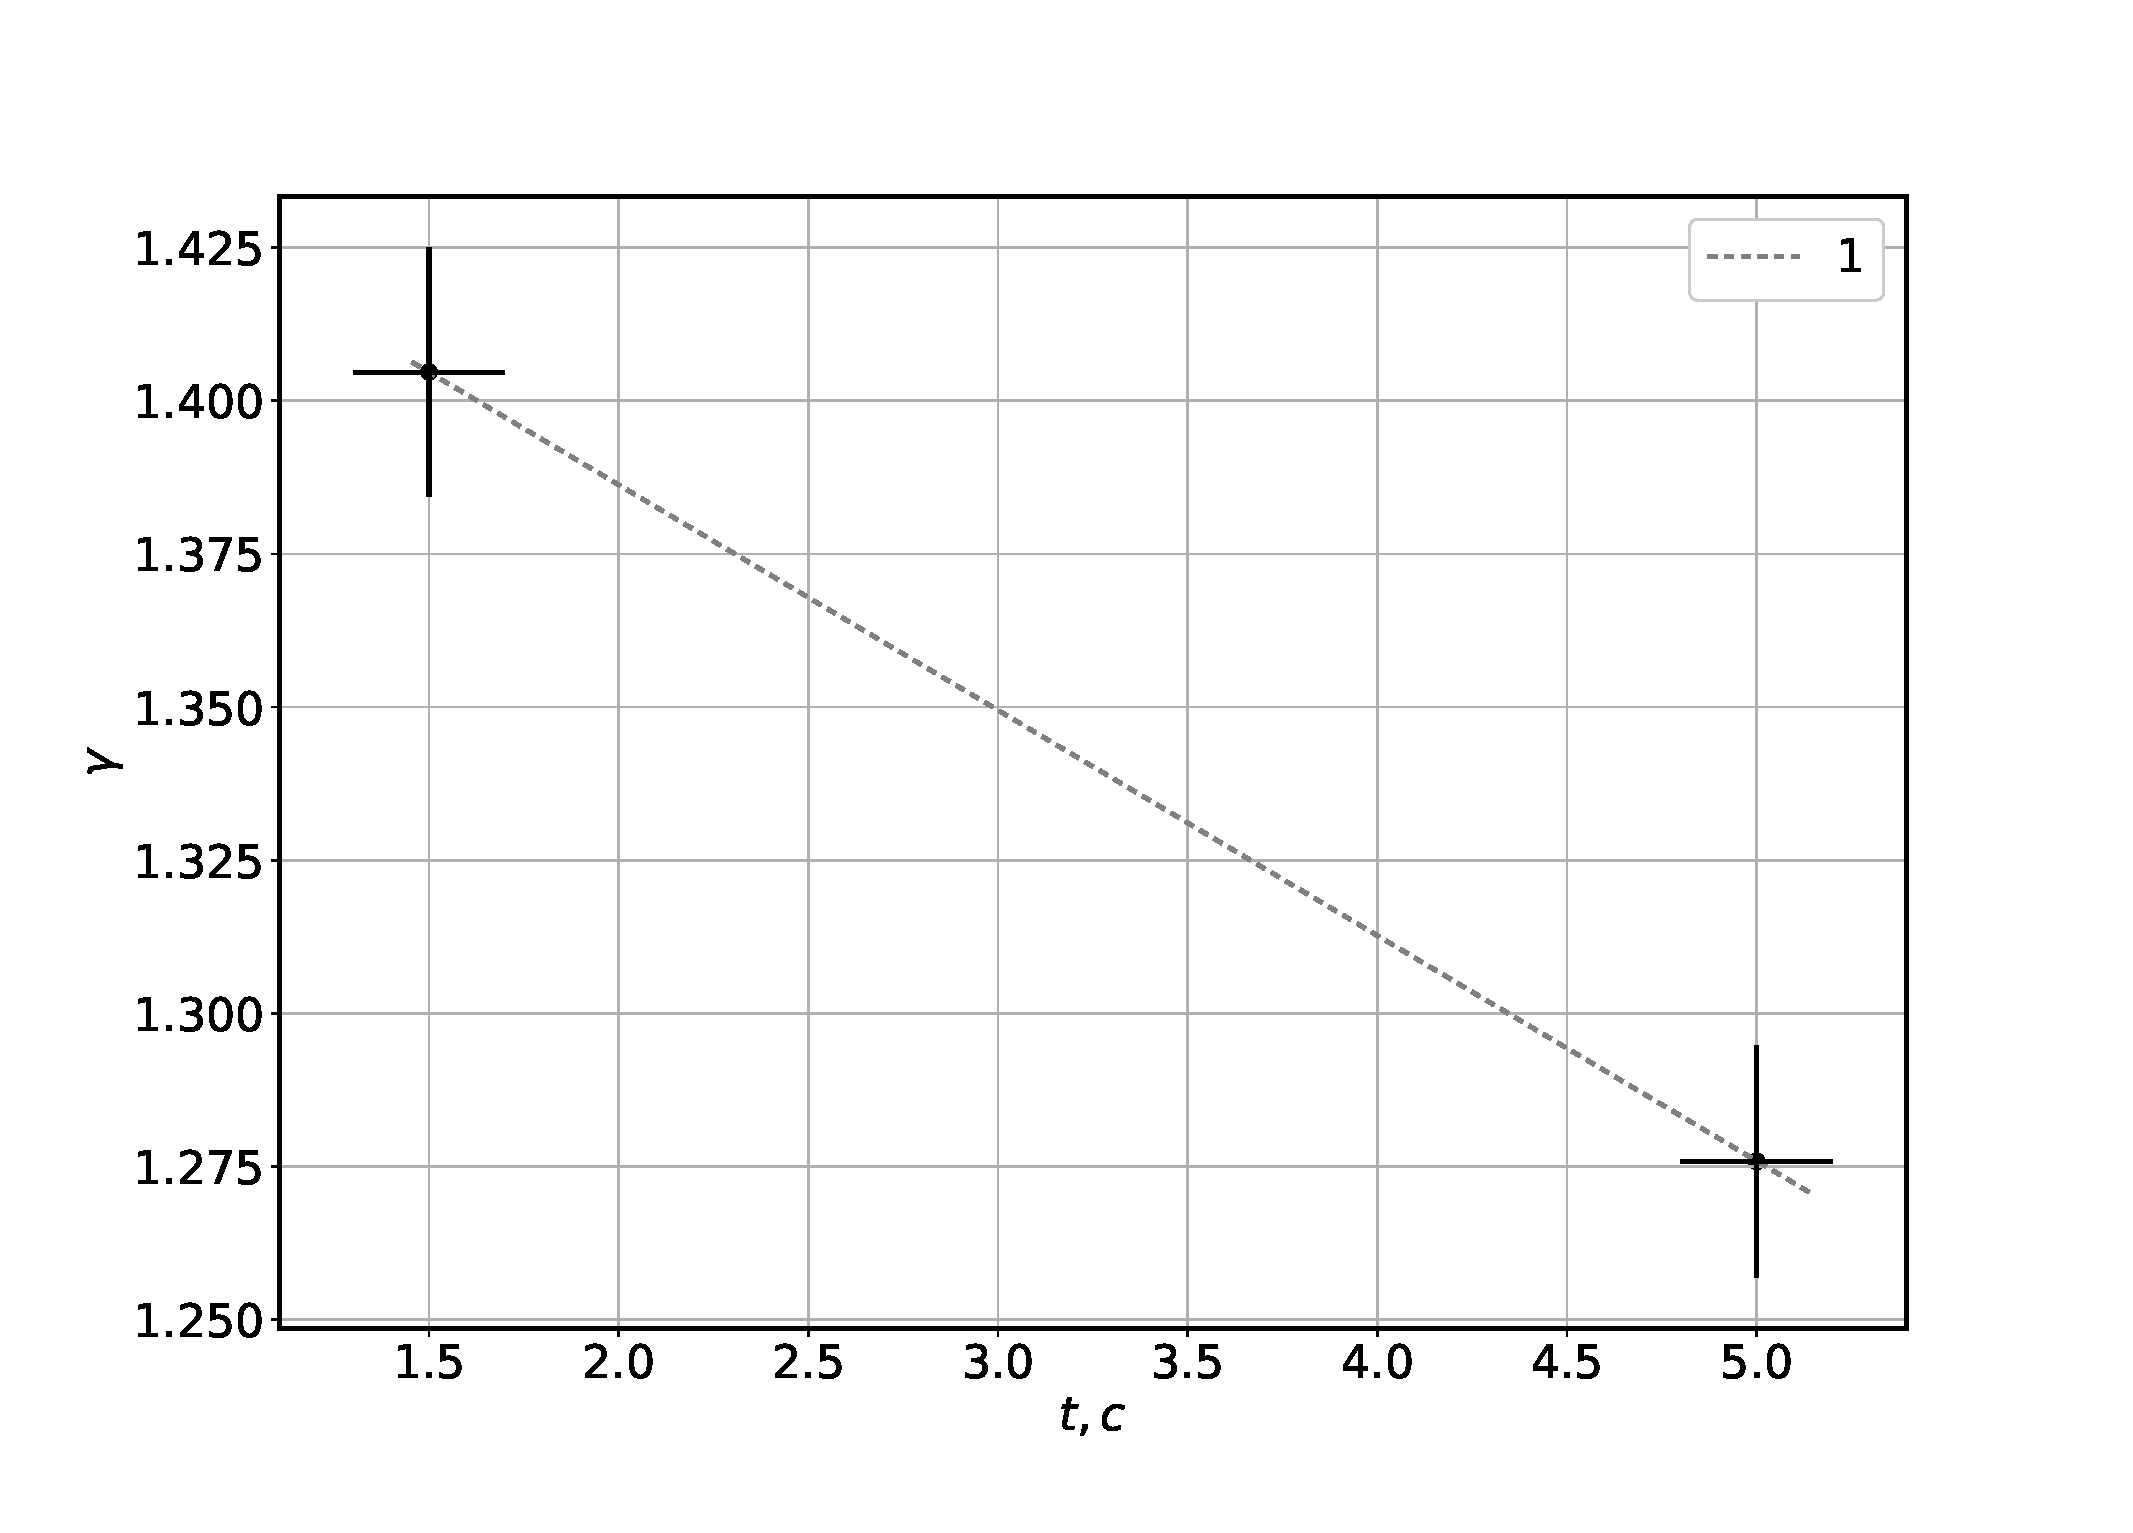
\includegraphics[width=0.7\linewidth]{gammat.eps}
    \caption{Зависимость покзателя адиабаты $\gamma$ от времени открытия клапана $t$.}
    \label{fig:2}
\end{figure}
Так как при увеличении времени открытия клапана мы получаем более заниженные результаты, для получения правильного 
значения следует аппроксимировать кривую до значения времени открытия клапана приблизительно $0.2$ с. 
Таким образом истинное значение показателя адиабаты равно $\gamma = 1.45 \pm 0.05$. Теоретическая
оценка показателя адиабаты двухатомного газа даёт значение $\gamma_T = 1.4$. Потому полученное в опыте 
значение можно считать корректным.  

\section{Выводы}
Проведен эксперимент по определению показателя адиабаты у углекислого газа методом адиабатического 
расширения. Полученное значение показателя адиабаты составило $\gamma = 1.45 \pm 0.05$. При этом 
теоретическая оценка показала $\gamma_T = 1.4$. Однако несмотря на совпадение результатов, был сделан вывод о 
несостоятельности данного метода измерения, так как погрешнность полученного значения составила $3\%$, 
тогда как показатели теплоёмкости двухатомного и трёхатомного газа отличаются всего на $4\%$. Потому 
представленный метод не может обеспечить нужную точность для измерения.    

\section{Использованная литература}
\begin{thebibliography}{9}
    \bibitem{LabBook}
    Лабораторный практикум по общей физике, Том 2, под редакцией А. Д. Гладуна
\end{thebibliography}

\section{Приложения}
\subsection{Параметры экспериментальной установки} \label{app_1}

\subsection{Данные результатов измерений} \label{app_2}
\begin{table}[H]
    \centering
    \begin{tabular}{|l|l|}
        \hline
        t, с & h, см \\ 
        \hline
        0    & 9.5   \\ 
        10   & 9.8   \\
        20   & 10.0  \\ 
        30   & 10.0  \\ 
        40   & 10.1  \\
        50   & 10.1  \\
        60   & 10.1  \\
        \hline
    \end{tabular}
    \caption{Данные результатов измерения установления высоты столба воды в сосуде $h$ от времени $t$.}
    \label{tab:1}
\end{table}

\begin{table}[H]
    \centering
    \begin{tabular}{|l|l|}
        \hline
        $h_1$, см & $h_2$, см  \\
        \hline
        9.7       & 13.7        \\ 
        9.8       & 13.7        \\ 
        9.8       & 13.3        \\ 
        9.9       & 13.4        \\ 
        10.0      & 13.5        \\ 
        9.8       & 13.5        \\ 
        9.9       & 13.5        \\ 
        \hline
    \end{tabular}
    \caption{Данные результатов измерения высот $h_1$ и $h_2$ столба жидкости при открывании крана
        приблизительно на $1.5$ с}
    \label{tab:2}
\end{table}
\begin{table}[H]
    \centering
    \begin{tabular}{|l|l|}
        \hline
        $h_1$, см & $h_2$, см \\ 
        \hline
        9.7       & 13.9      \\ 
        9.9       & 13.9      \\ 
        9.8       & 13.8      \\ 
        9.9       & 13.9      \\ 
        9.8       & 13.9      \\ 
        \hline
    \end{tabular}
    \caption{Данные результатов измерения высот $h_1$ и $h_2$ столба жидкости при открывании крана
        приблизительно на $5$с}
    \label{tab:3}
\end{table}

\end{document}